\subsection{Background}
Both neural networks and fuzzy systems have some things in common. They can be used for solving a problem (e.g. pattern recognition, regression or density estimation) if there does not exist any mathematical model of the given problem. They solely do have certain disadvantages and advantages which almost completely disappear by combining both concepts.

Neural networks can only come into play if the problem is expressed by a sufficient amount of observed examples. These observations are used to train the black box. On the one hand no prior knowledge about the problem needs to be given. On the other hand, however, it is not straightforward to extract comprehensible rules from the neural network's structure.

On the contrary, a fuzzy system demands linguistic rules instead of learning examples as prior knowledge. Furthermore the input and output variables have to be described linguistically. If the knowledge is incomplete, wrong or contradictory, then the fuzzy system must be tuned. Since there is not any formal approach for it, the tuning is performed in a heuristic way. This is usually very time consuming and error-prone.

\begin{table}[h]
\centering
    \begin{tabular}{ | l | l | }
	    \hline
	    \rowcolor{gray!20}
		\multicolumn{1}{|c|}{\textbf{Neural Networks}} & \multicolumn{1}{|c|}{\textbf{Fuzzy Systems}} \\ \hline % multicolumn makes it center with |c|
		%\textbf{Neural Networks} & \textbf{Fuzzy systems}\\ \hline
	    no mathematical model necessary & no mathematical model necessary\\ \hline
	    learning from scratch & apriori knowledge necessary \\ \hline
	    several learning algorithm & not capable to learn \\ \hline
	    black box behavior & simple interpretation and implementation \\ \hline
    \end{tabular}
    \caption{Comparison of neural networks and fuzzy systems}
    \label{tab:comparison_neur_ann}
\end{table}

As shown in the table ~\ref{tab:comparison_neur_ann} we can see that fuzzy systems and neural networks have quite contrary traits which connected can create a very powerful system.

\subsection{Fuzzy logic}
There are many misconceptions about fuzzy logic.
Fuzzy logic is not fuzzy.
Basically, fuzzy logic is a precise logic of imprecision and approximate reasoning.

In real world, we do not assign precise parameters or criteria to most objects that we encounter on every day basis.

\begin{wrapfigure}{r}{0.6\textwidth}
	\captionsetup{width=18pc}
	\vspace*{-2em}
	\hspace*{1.5em}
	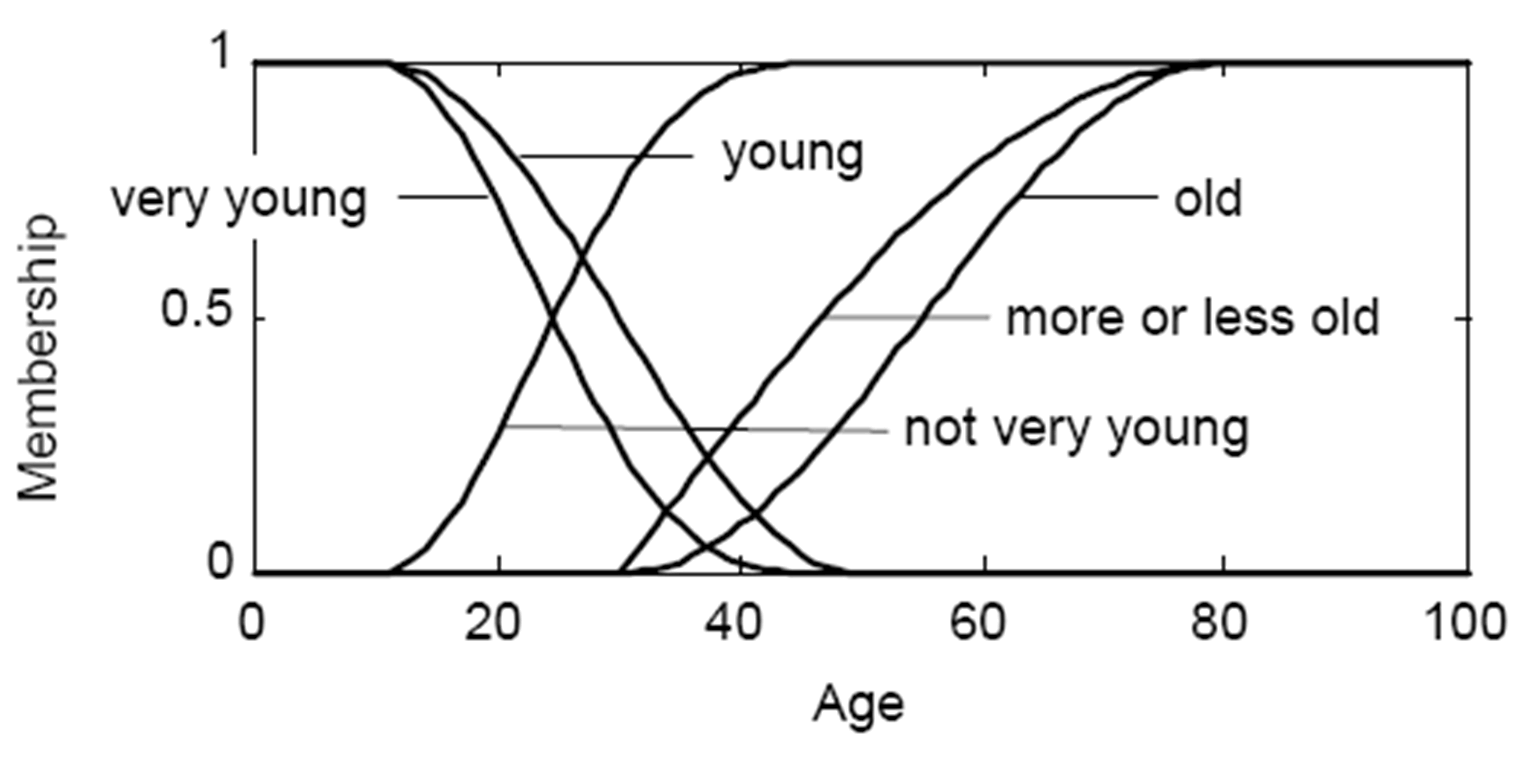
\includegraphics[width=0.5\textwidth]{images/old_graph.png}
	%[height=0.4\textheight,keepaspectratio]
	\caption{Usage of linguistic variable while describing someone's age~\cite{lecture_rome_university}}
	\label{fig:old_graph}
	\vspace*{-2em}
\end{wrapfigure}

For instance describing someone's age one can say that a person being 50 years old is \emph{old} but someone else may consider that person as \emph{middle-aged}.
This is what we call fuzzy logic \emph{linguistic variable}.
In Figure~\ref{fig:old_graph} one can see that to each linguistic variable a \emph{membership function} is assigned with yields for each age it's membership rate from 0 to 1.
People do not acknowledge that in everyday usage, they just use it and take it for granted.
Computers have hard time describing those type of traits in a descriptive manner as was shown with age example.

That's where fuzzy logic comes in hand.
Although fuzzy logic has been studied since 1920s (as study of infinite-valued logic), the term ``fuzzy sets'' has been coined by Lofti A. Zadeh, a professor at the University of California at Berkley in his article ``Fuzzy sets'' in 1965 \cite{fuzzy_sets_zadeh} as a mean to model the uncertainty
of natural language.
He was trying to argument for his idea saying that people do not require precise, numerical information input, and yet they are capable of highly adaptive control and if one had been able to program a system to accept noisy, imprecise input it would have been much more effective than contemporary systems.

Fuzzy systems:
\begin{itemize}
\item Are inherently robust since they do not require precise, noise-free inputs and can be programmed to fail safely if a feedback sensor quits or is destroyed. The output control is a smooth control function despite a wide range of input variations,
\item Are not limited to few feedback inputs and one or two outputs, nor is it necessary to measure or compute rate-of-change parameters in order for it to be implemented. Any control data that provides some indication of system's actions and reactions is sufficient. This allows the fuzzy systems to be inexpensive and imprecise thus keeping the overall system cost and complexity low,
\item Since fuzzy logic controller processes user-defined rules governing the target control system, it can be modified and tweaked easily to improve or drastically alter system performance. New sensors can easily be incorporated into the system simply by generating appropriate governing rules,
\item Because of the rule-based operation, any reasonable number of inputs can be processed and numerous outputs generated, although defining the rulebase quickly becomes complex if too many inputs and outputs are chosen for a single implementation since rules defining their interrelations must also be defined. It would be better to break the system into smaller chunks and use several smaller fuzzy controllers distributed on the system, each with more limited responsibilities,
\item Fuzzy systems can control nonlinear systems that would be difficult or impossible to model mathematically. This opens doors for control systems that would normally be deemed unfeasible for automation.
\end{itemize}

\clearpage
\subsection{Artificial Neural Networks}
Having nowadays ``traditional'' computer systems we can use it efficiently to some extent in various scenarios and for various purposes, e.g. multimedia systems, video games, document editing, algebra or arithemics.

\begin{table}[h]
\centering
    \begin{tabular}{ | l | l | }
	    \hline
	    \rowcolor{gray!20}
		\multicolumn{2}{|c|}{\textbf{Everyday computer systems}} \\ \hline % multicolumn makes it center with |c|
	    \rowcolor{gray!35}
		\multicolumn{1}{|c|}{\textbf{Good at}} & \multicolumn{1}{|c|}{\textbf{Not so good at}} \\ \hline % multicolumn makes it center with |c|
	    fast arithmetic & massive parallelism \\ \hline
	    precisely executing programmed commands & working with noisy inputs \\ \hline
	    \multicolumn{1}{|c|}{-} & adapting to tolerances \\ \hline
	    \multicolumn{1}{|c|}{-} & adapting to changing curcumstances\\ \hline
    \end{tabular}
    \caption{Traits of everyday, traditional computer systems.~\cite{intro_ann_leslie_smith}}
    \label{tab:everyday_computer_systems}
\end{table}Artificial neural networks are computational models inspired by human's brain, that are capable of machine learning and pattern recognition.

When some more abstract human like processing comes to play like defining a structure/model based on a concrete data set, prediction based on an example set then traditional computers start to pant.
That's were artificial neural networks come to place.


Artificial neural networks are usually presented as systems of interconnected ``neurons'' (just like human brain's neurons, hence the name), that can compute values from inputs by feeding information through the network.


\begin{wrapfigure}{r}{0.48\textwidth}
	\vspace*{-2.5em}
	\hspace*{1em}
	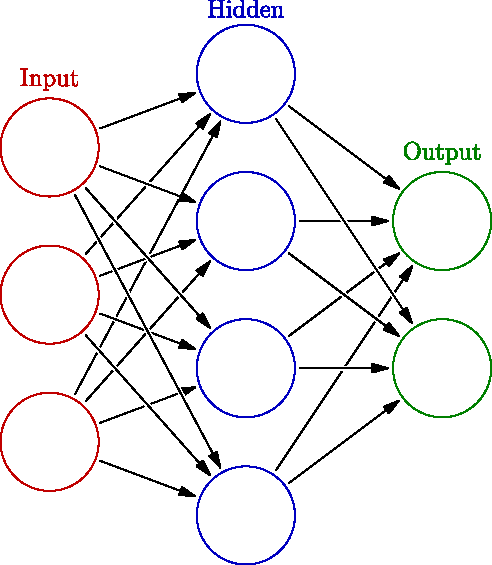
\includegraphics[width=0.44\textwidth]{images/ann_wiki_model.pdf}
	%[height=0.4\textheight,keepaspectratio]
	\caption{Artificial neural network model showing its free layers: inputs, hidden layer and output layer.~\cite{wiki_ann}}
	\label{fig:ann_model}
\end{wrapfigure}

They use learning algorithms that are inspired by understanding of how the brain learns, but they are evaluated by how well they work for practical applications such as speech recognition, object recognition, image retrieval and the ability to recommend products that a user will like.
Despite being quite powerful when properly designed artificial neural networs are orders of magnitude less complex than human brains.
As computers become more powerful, artificial neural networks are gradually taking over from simpler machine learning methods.
They are already at the heart of a new generation of speech recognition devices and they are beginning to outperform earlier systems for recognizing objects in images.

\vspace*{5em}

